\documentclass{roadef}

\title{Un vaste voisinage pour le problème de tournées de véhicules}

\author{Guillaume Pinot}

\institute{
  Kardinal, Paris, France\\
  \email{guillaume.pinot@kardinal.ai}
}

\begin{document}

\maketitle

\keywords{tournées de véhicules, recherche locale, voisinage,
  regroupement hiérarchique}

\section{Introduction}

Le problème de tournées de véhicules est un problème d'optimisation
combinatoire NP-difficile classique aux nombreuses variantes et aux
nombreuses applications industrielles. Le but est de générer les
tournées d'une flotte de véhicules afin de réaliser des visites de
clients.

Les approches de résolution les plus répandues pour ces problèmes sont
des méthodes de recherche locale. À partir d'une solution réalisable,
un voisinage est défini, modélisant un ensemble de solutions
réalisables semblables à la première. Dans ce voisinage, une solution
est choisie, souvent de bonne qualité, parfois simplement la
meilleure.

Chez Kardinal, nous traitons des problèmes de tournées de véhicules
très riches et très différents. La richesse des contraintes rend
l'utilisation des méthodes exactes très complexes, c'est pourquoi nous
nous sommes tournés vers les méthodes de recherche locale. Bien que
rapides et efficaces dans la plupart des cas, elles ont leurs limites:
elles sont rarement efficaces pour la minimisation du nombre de
véhicules. C'est pourquoi nous nous sommes penchés sur la génération
de voisinages plus vastes, afin de pouvoir répondre, entre autres, à
cette problématique.

\section{Problème de partitionnement}

Le problème de tournées de véhicules se découpe naturellement en deux:
le problème des tournées isolées (que l'on peut voir comme un problème
de voyageur de commerce) et le problème de partitionnement des clients
sur les véhicules. Cette modélisation est au cœur de la modélisation
en programmation linéaire, mais est également très présente dans les
algorithmes de recherche locale.

Dans le reste de cet article, nous nous focaliserons sur le problème
de partitionnement. Nous supposerons que nous avons à notre
disposition un algorithme permettant de valider l'affectation d'un
ensemble de clients à un véhicule et de donner les caractéristiques
de la tournée correspondante (distance parcourue, somme des retards,
\emph{etc.}). Un tel algorithme est facile à obtenir en utilisant de
simples tests pour valider les contraintes et des heuristiques pour
trouver une tournée de bonne qualité, comme une procédure 2-opt.

\section{Problématique}

Les mouvements très simples sur le problème de partitionnement, comme
le déplacement d'un client d'une tournée à une autre, permettent
d'obtenir rapidement et facilement une solution de qualité
correcte. Le minimum local ainsi trouvé peut souvent être grandement
amélioré. Au regard d'une telle solution, déplacer les clients par
groupe plutôt que un à un semble judicieux.

Faire de tels mouvements complexifie grandement la procédure. La
difficulté est de trouver un voisinage suffisamment large pour sortir
des minima locaux, suffisamment cohérent pour décrire un grand ensemble
de solutions et suffisamment petit pour être exploitable.

\section{Le voisinage}

Le voisinage est décrit par un ensemble de tournées candidates. Un
programme linéaire est ensuite généré sur ces tournées (chaque client
doit être visité exactement une fois). Le programme linéaire est
ensuite résolu par un solveur linéaire, après injection de la solution
courante comme solution initiale.

Les tournées candidates sont toutes les tournées réalisables tel qu'un
groupe de clients a été enlevé et/ou ajouté à une tournée existante.

Les groupes de clients sont générés en se basant sur la solution
courante. Pour chaque tournée de la solution courante, un regroupement
hiérarchique est généré sur l'échelle temporelle des visites des
clients. La distance utilisée correspond à la durée nécessaire pour
réaliser le groupe de clients dans la tournée. Chaque nœud de l'arbre
représente un groupe de clients. Ainsi, nous avons une grande
diversité de tailles de groupes, allant des groupes d'un client au
groupe composé de tous les clients de la tournée. La structure
arborescente générée par le regroupement hiérarchique permet également
les recombinaisons complexes, comme chaque groupe peut être découpé en
deux groupes de manière hiérarchique.

Le voisinage ainsi décrit est très grand, mais sa structure rend la
résolution relativement facile pour les solveurs linéaires
modernes. La structure hiérarchique des groupes permet des
recombinaisons complexes, permettant de supprimer des véhicules. La
figure~\ref{fig:mouvements} permet de visualiser le chemin d'une
solution obtenue avec un algorithme glouton à 9~véhicules jusqu'à la
solution optimale en 3~véhicules en effectuant seulement 5 mouvements.

\begin{figure}[htbp]
  \centering
  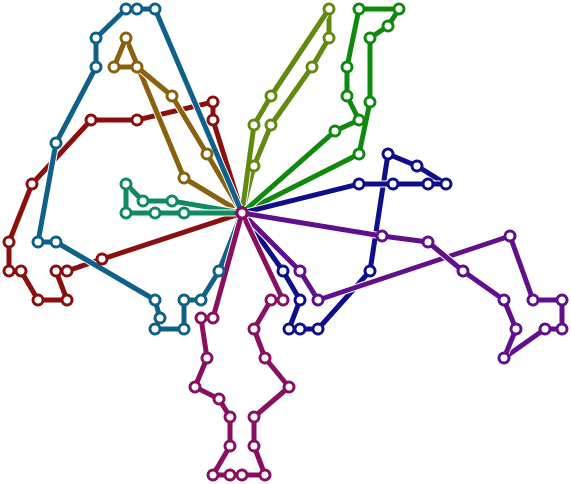
\includegraphics[width=0.33\linewidth]{images/C203-0}\hfill
  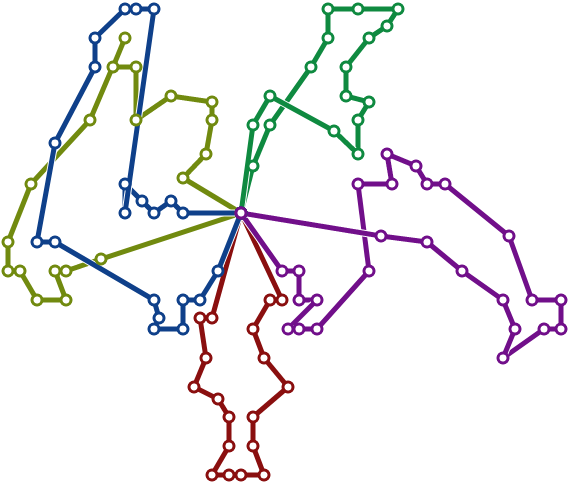
\includegraphics[width=0.33\linewidth]{images/C203-1}\hfill
  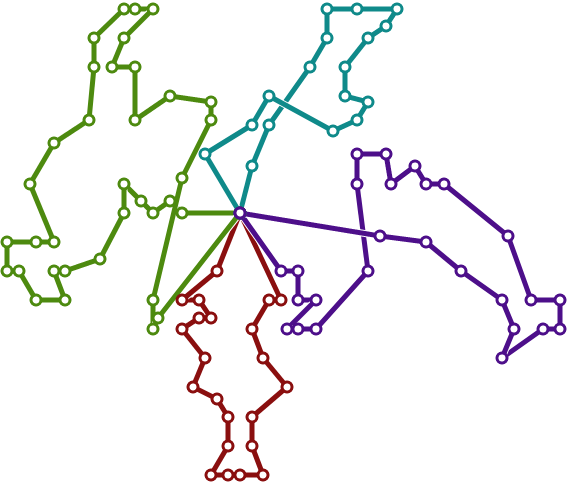
\includegraphics[width=0.33\linewidth]{images/C203-2}\hfill
  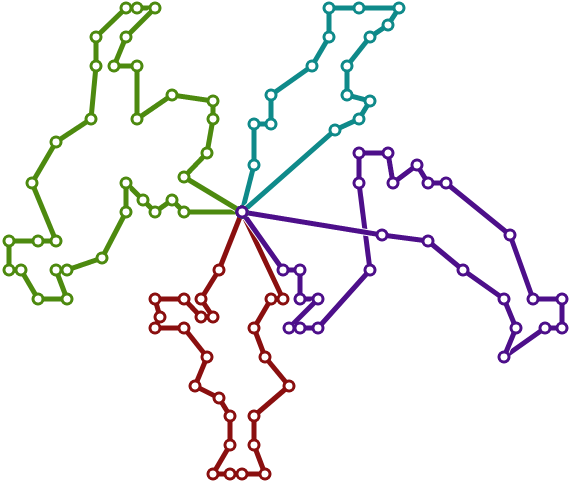
\includegraphics[width=0.33\linewidth]{images/C203-3}\hfill
  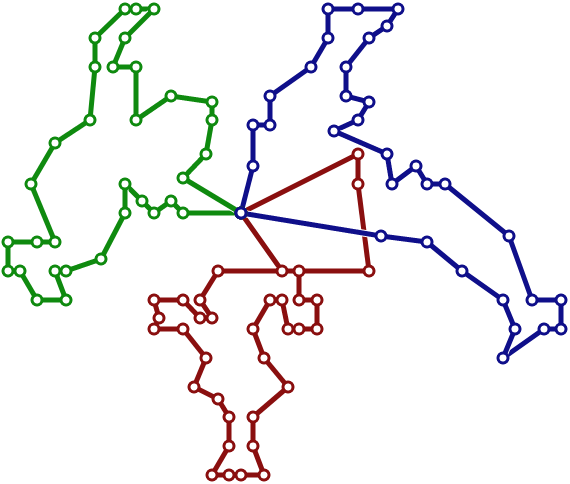
\includegraphics[width=0.33\linewidth]{images/C203-4}\hfill
  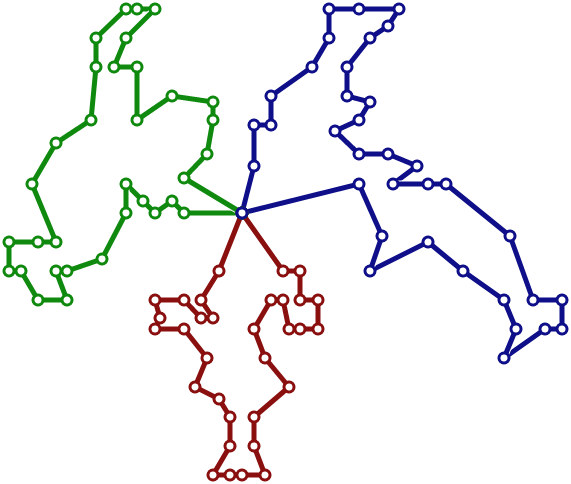
\includegraphics[width=0.33\linewidth]{images/C203-5}

  \caption{D'un minimum local à l'optimal en 5 mouvements sur une
    instance VRPTW de la littérature}
  \label{fig:mouvements}
\end{figure}

\section{Conclusions et perspectives}

Cet article présente un grand voisinage pour le problème de tournées
de véhicules. Les premières expérimentations sur des instances de la
littérature ainsi que sur des instances réelles sont prometteuses,
particulièrement en support d'une recherche locale simple.

Le critère utilisé dans le regroupement hiérarchique doit pouvoir être
amélioré pour mieux prendre en compte les différents objectifs et
contraintes du problème.

\end{document}
